\section{错误处理}
错误处理是 C++ 的一项关键功能。 本章讨论将工作卸载到设备(加速器)时遇到的独特错误处理挑战,
以及 SYCL 如何使我们完全可以应对这些挑战。

检测和处理意外情况和错误在应用程序开发过程中很有帮助(想想:从事该项目的其他程序员确实会犯错误),
但更重要的是在稳定和安全的生产应用程序和库中发挥关键作用。 
本章致力于描述 C++ 中可用的 SYCL 错误处理机制,以便我们能够了解我们的选项是什么,
以及如果我们关心检测和管理错误,如何构建应用程序。

本章概述了 SYCL 中的同步和异步错误,描述了如果我们在代码中不执行任何操作来处理错误,
应用程序的行为,并深入探讨允许我们处理异步错误的 SYCL 特定机制。


\subsection{安全第一}
C++ 错误处理的一个核心方面是,如果我们不采取任何措施来处理已检测到(引发)的错误,那么应用程序将终止并指示出现问题。 
这种行为使我们能够在编写应用程序时无需关注错误管理,并且仍然确信错误会以某种方式向开发人员或用户发出信号。 
当然,我们并不是建议我们应该忽略错误处理! 生产应用程序的编写应将错误管理作为架构的核心部分,
但应用程序在开始开发时通常没有这样的关注点。 
C++ 的目标是使不处理错误的代码仍然能够观察到许多错误,即使它们没有被显式处理。

由于 SYCL 是数据并行 C++,因此同样的理念成立:如果我们在代码中不采取任何措施来管理错误,并且检测到错误,
则程序将发生异常终止,让我们知道发生了错误。 生产应用程序当然应该将错误管理视为软件架构的核心部分,不仅要报告,
而且通常还要从错误情况中恢复。

\begin{remark}
	如果我们不添加任何错误管理代码并且发生错误,我们仍然会看到程序异常终止,这表明需要进行更深入的研究。
\end{remark}

\subsection{错误类型}
C++ 通过其异常机制提供了一个用于通知和处理错误的框架。 
除此之外,异构编程还需要额外级别的错误管理,因为设备上或尝试在设备上启动工作时会发生一些错误。 
这些错误通常与主机程序的执行及时分离,因此它们不能与常规 C++ 异常处理机制干净地集成。 
为了解决这个问题,有额外的机制可以使异步错误像典型的 C++ 异常一样易于管理和控制。

\begin{figure}[H]
	\centering
	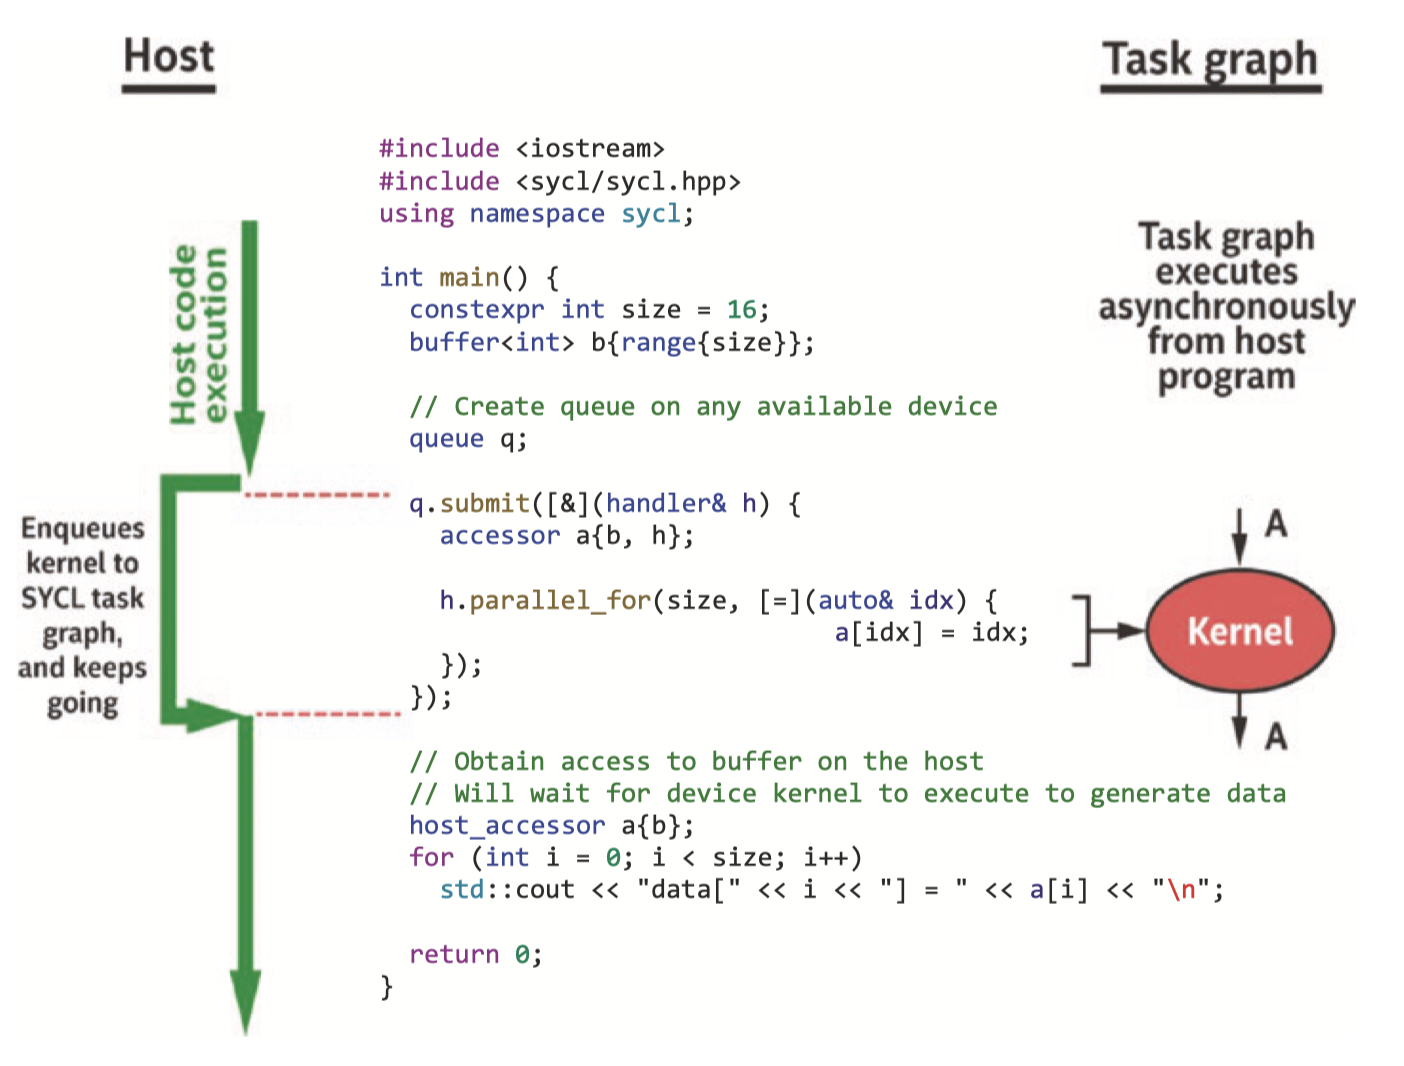
\includegraphics[width=0.9\textwidth]{figs/F5.1.png}
	\caption{\textit{主机程序和任务图执行的分离}}
\end{figure}

图 5-1 显示了典型应用程序的两个组件:(1) 主机代码按顺序运行并将工作提交到任务图以供将来执行;
(2) 任务图与主机程序异步运行并执行Kernel或其他程序 当满足必要的依赖性时对设备执行的操作。 
该示例显示了parallel\_for作为任务图的一部分异步执行的操作,但其他操作也是可能的,并在第3、4和8章中讨论。

图 5-1 左右(主机和任务图)之间的区别是理解同步错误和异步错误之间差异的关键。

当主机程序执行操作(例如 API 调用或对象构造)时检测到错误条件时,就会发生同步错误。 
它们可以在图左侧的指令完成之前被检测到,并且导致错误的操作可以立即抛出错误。 
我们可以使用 try-catch 构造将特定指令包装在图的左侧,
期望在 try 块结束之前检测到由于 try 内的操作而发生的错误(并因此捕获)。 
C++ 异常机制旨在准确处理这些类型的错误。

异步错误发生在图 5-1 右侧的部分,只有在执行任务图中的操作时才会检测到错误。 
当异步错误作为任务图执行的一部分被检测到时,主机程序通常已经继续执行,
因此没有代码可以用 try-catch 结构包装来捕获这些错误。 
相反,SYCL 中有一个异步异常处理框架来处理这些相对于主机程序执行看似随机且不受控制的时间发生的错误。

\subsection{让我们创建一些错误!}
作为本章剩余部分的示例并允许我们进行实验,我们将在以下示例中创建同步和异步错误。

\subsubsection{同步错误}
\begin{figure}[H]
	\centering
	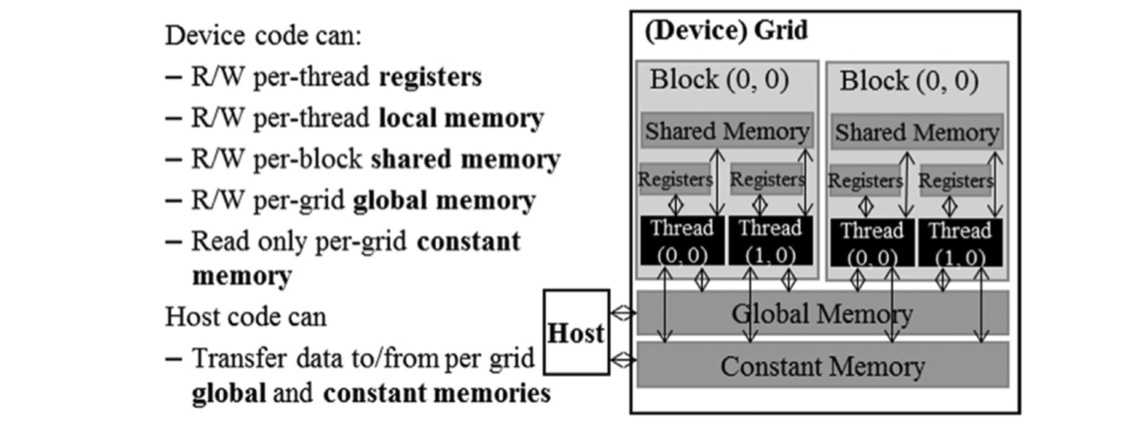
\includegraphics[width=0.9\textwidth]{figs/F5.2.png}
	\caption{\textit{创建同步错误}}
\end{figure}

在图 5-2 中,从缓冲区创建了一个子缓冲区,但其大小非法(大于原始缓冲区)。 
子缓冲区的构造函数检测到此错误并在构造函数执行完成之前抛出异常。 
这是一个同步错误,因为它是作为主机程序执行的一部分(同步)发生的。 
在构造函数返回之前可以检测到错误,因此可以在错误的起源点或在主机程序中检测到错误时立即对其进行处理。

我们的代码示例没有执行任何操作来捕获和处理 C++ 异常,
因此默认的 C++ 未捕获异常处理程序为我们调用 std::terminate,表示出现了问题。

\subsubsection{异步错误}
\begin{figure}[H]
	\centering
	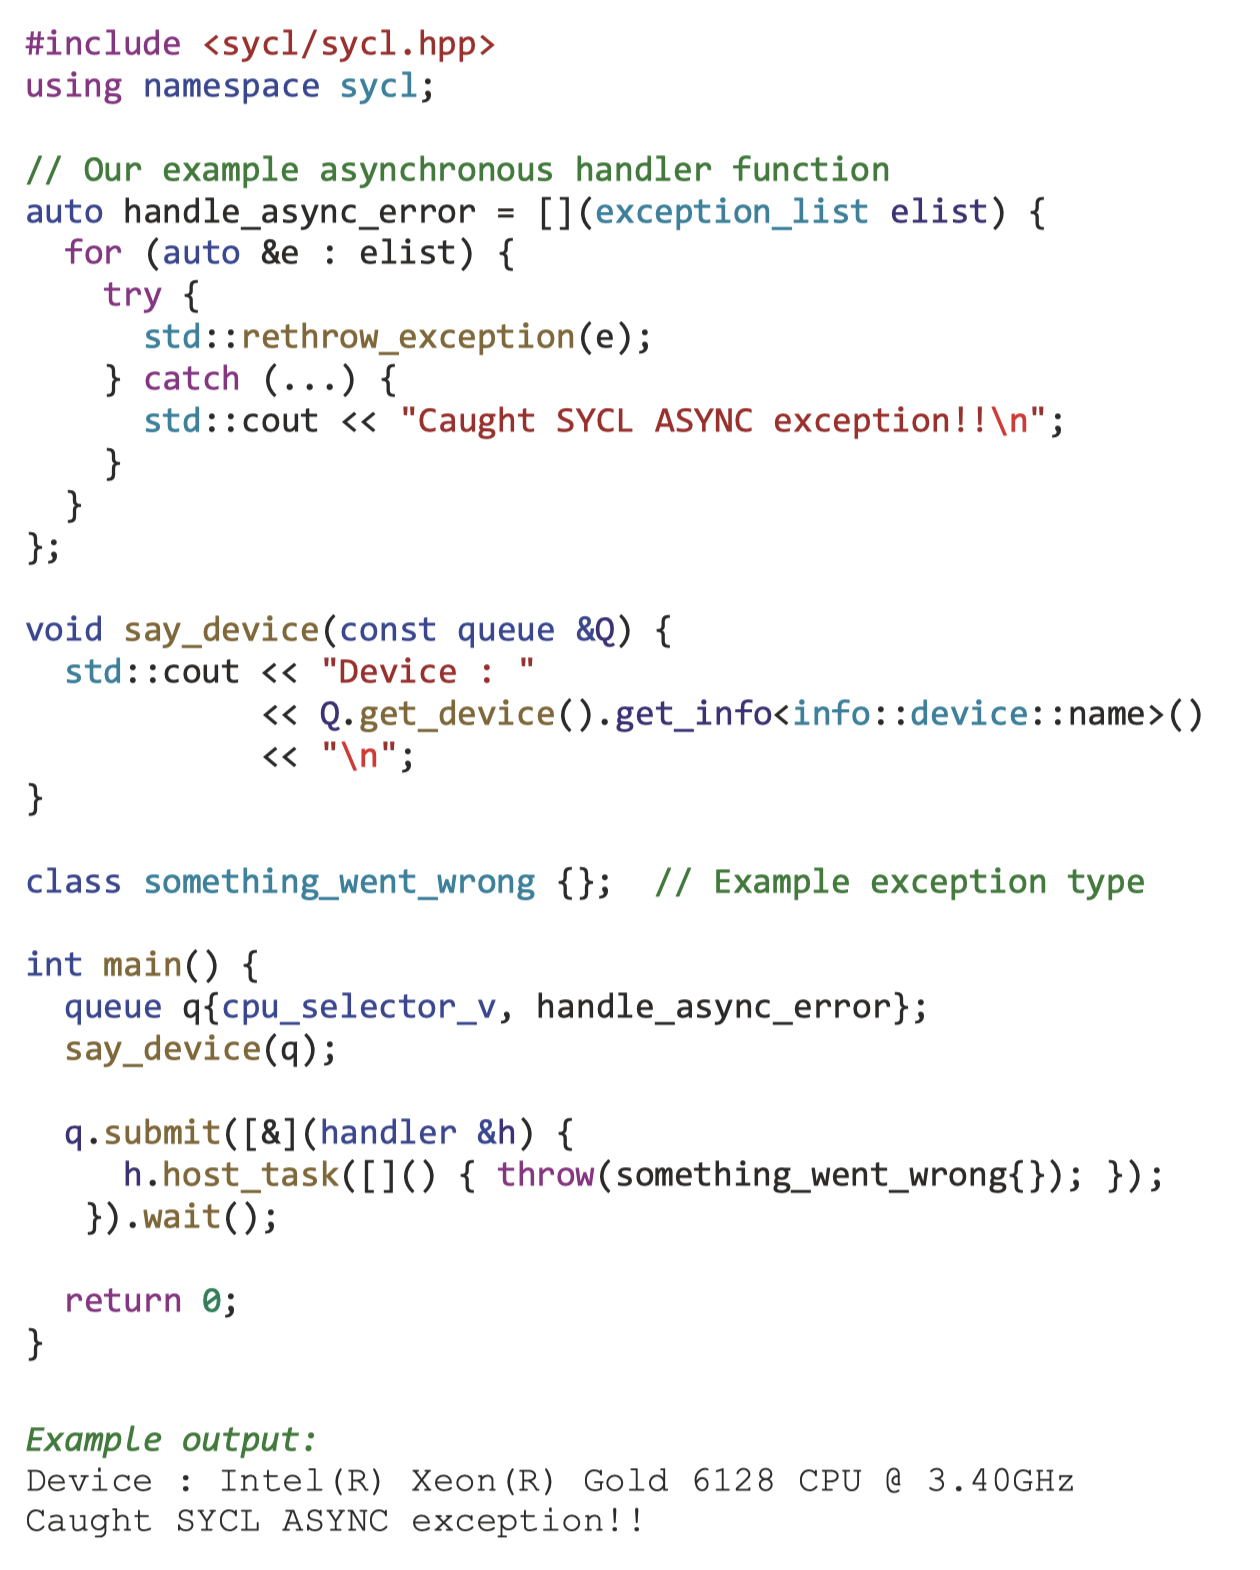
\includegraphics[width=0.9\textwidth]{figs/F5.3.png}
	\caption{\textit{创建异步错误}}
\end{figure}

生成异步错误有点棘手,因为实现会尽可能努力同步检测和报告错误。 
同步错误更容易调试,因为它们发生在主机程序中的特定起始点,因此只要有可能,它们都是实现的首选。 
出于演示目的,生成异步错误的一种方法是在主机任务内引发异常,该任务作为任务图的一部分异步执行。 
图 5-3 演示了此类异常。 异步错误在许多情况下都可能发生并报告,因此请注意,
图 5-3 中所示的主机任务示例只是一种可能性,而不是异步错误的要求。

\subsection{应用程序错误处理策略}
C++ 异常功能旨在将程序中检测到错误的点与可能处理错误的点清楚地分开,并且此概念非常适合 SYCL 中的同步错误和异步错误。 
通过抛出和捕获机制,可以定义处理程序的层次结构,这在生产应用程序中非常重要。

构建能够以一致且可靠的方式处理错误的应用程序需要预先制定策略以及为错误管理而构建的软件架构。 
C++ 提供了灵活的工具来实现许多替代策略,但这种架构超出了本章的范围。 
有许多书籍和其他参考文献专门讨论此主题,因此我们鼓励您查阅它们以全面了解 C++ 错误管理策略。

也就是说,错误检测和报告并不总是需要达到生产规模。 如果目标只是在执行期间检测错误并报告错误(但不一定要从中恢复),
则可以通过最少的代码可靠地检测和报告程序中的错误。 
以下各节首先介绍如果我们忽略错误处理并且不执行任何操作(默认行为并没有那么糟糕!)会发生什么,
然后是在基本应用程序中易于实现的推荐错误报告。

\subsubsection{忽略错误处理}
C++ 和 SYCL 旨在告诉我们,即使我们没有显式处理错误,也会出现问题。 
未处理的同步或异步错误的默认结果是程序异常终止,操作系统应该告诉我们这一点。 
以下两个示例分别模拟了如果我们不处理同步错误和异步错误时将发生的行为。

\begin{figure}[H]
	\centering
	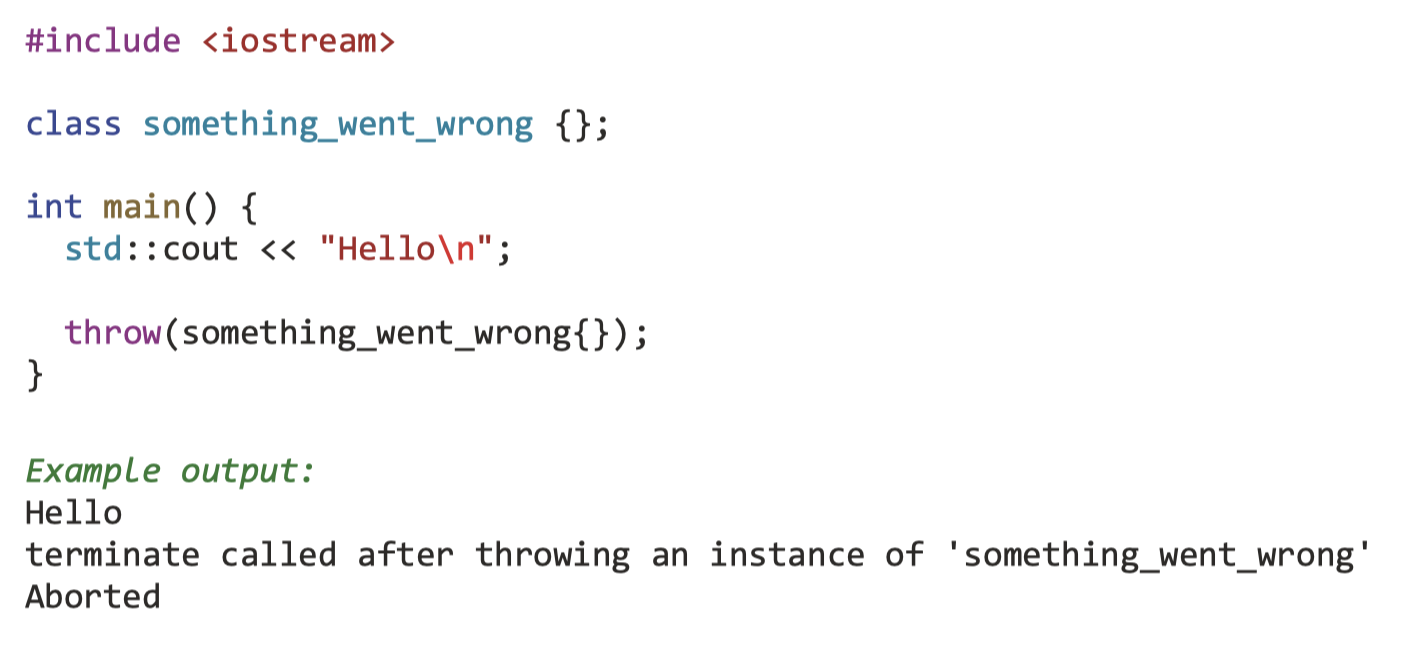
\includegraphics[width=0.9\textwidth]{figs/F5.4.png}
	\caption{\textit{C++ 中未处理的异常}}
\end{figure}

图 5-4 显示了未处理的 C++ 异常的结果,例如,该异常可能是未处理的 SYCL 同步错误。 
我们可以使用此代码来测试特定操作系统在这种情况下会报告什么。

\begin{figure}[H]
	\centering
	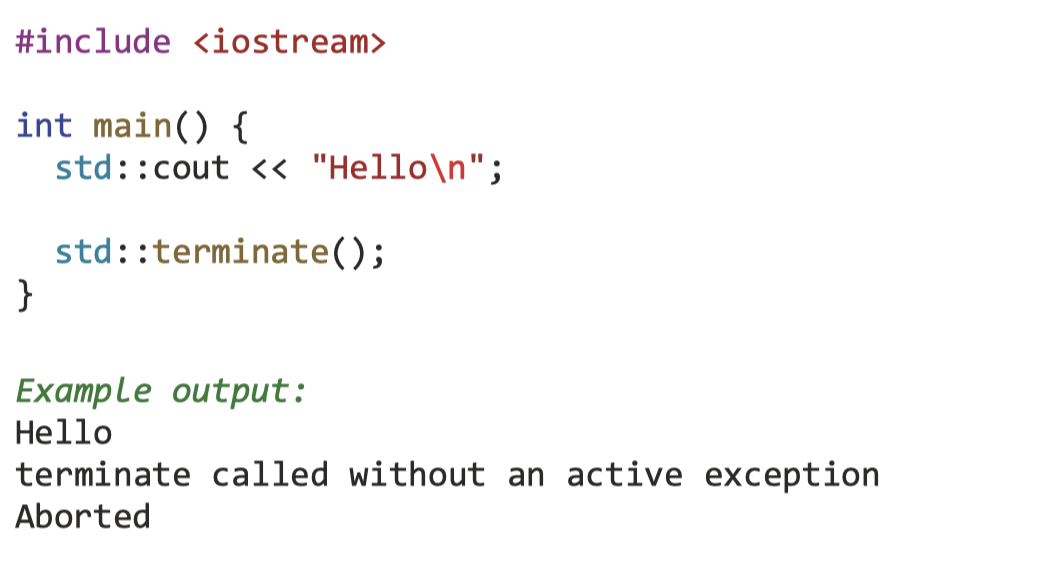
\includegraphics[width=0.9\textwidth]{figs/F5.5.png}
	\caption{\textit{std::terminate 在未处理 SYCL 异步异常时调用}}
\end{figure}

图 5-5 显示了调用 std::terminate 的示例输出,这将是我们的应用程序中未处理的 SYCL 异步错误的结果。 
我们可以使用此代码来测试特定操作系统在这种情况下会报告什么。

尽管我们应该处理程序中的错误,但未捕获的异常最终会被捕获并终止程序,这比异常被默默地丢失要好!

\subsubsection{同步错误处理}
我们将本节保持得非常简短,因为 SYCL 同步错误只是 C++ 异常。 
SYCL 中添加的大多数附加错误机制与我们在下一节中介绍的异步错误相关,
但同步错误很重要,因为实现尝试同步检测和报告尽可能多的错误,因为它们更容易推理和处理。

\begin{figure}[H]
	\centering
	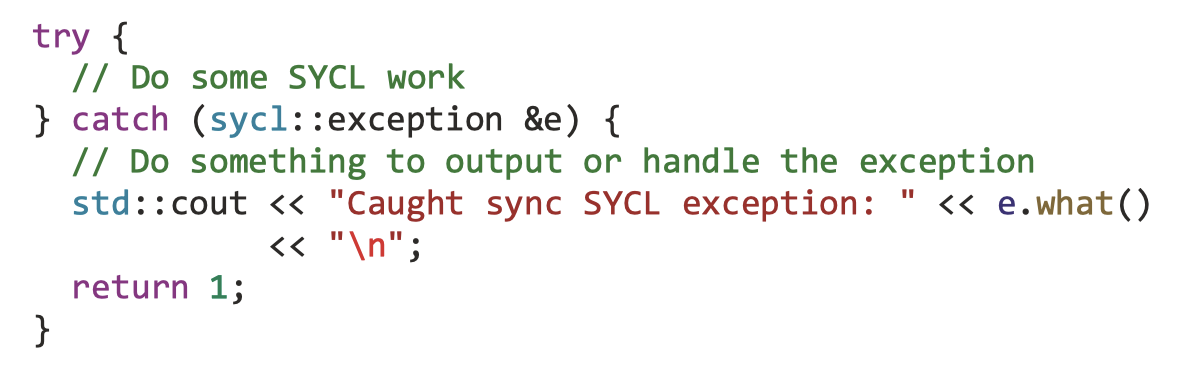
\includegraphics[width=0.9\textwidth]{figs/F5.6.png}
	\caption{\textit{专门捕获 sycl::exception 的模式}}
\end{figure}

SYCL 定义的同步错误属于 sycl::exception 类型,它是一个从 std::exception 派生的类,
它允许我们通过 try-catch 结构专门捕获 SYCL 错误,如图 5-6 所示。

在 C++ 错误处理机制之上,SYCL 为运行时抛出的异常添加了 sycl::exception 类型。 
其他一切都是标准 C++ 异常处理,因此大多数开发人员都会熟悉。

\begin{figure}[H]
	\centering
	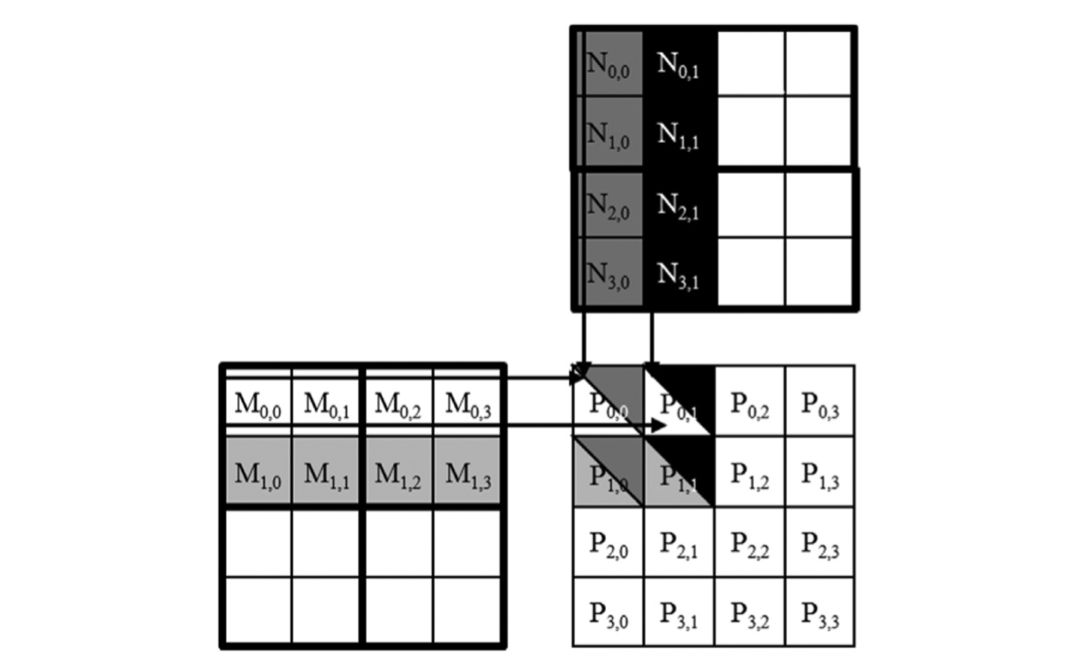
\includegraphics[width=0.9\textwidth]{figs/F5.7.png}
	\caption{\textit{从代码块中捕获异常的模式}}
\end{figure}

图 5-7 中提供了一个稍微更完整的示例,其中处理了其他类别的异常。

\subsubsection{异步错误处理}
异步错误由 SYCL 运行时(或底层后端)检测,并且错误的发生独立于主机程序中命令的执行。 
错误存储在 SYCL 运行时内部的列表中,并且仅在程序员可以控制的特定点释放以进行处理。 
我们需要讨论两个主题来讨论异步错误的处理:

\begin{enumerate}
	\item 当处理未完成的异步错误时,处理程序应该做什么
	\item 当异步处理程序被调用时
\end{enumerate}

\subsubsection{异步处理程序}
异步处理程序是应用程序定义的函数,它注册到 SYCL 上下文和/或队列。 
在下一节定义的时间,如果有任何未处理的异步异常可供处理,则 SYCL 运行时将调用异步处理程序并传递这些异常的列表。

\begin{figure}[H]
	\centering
	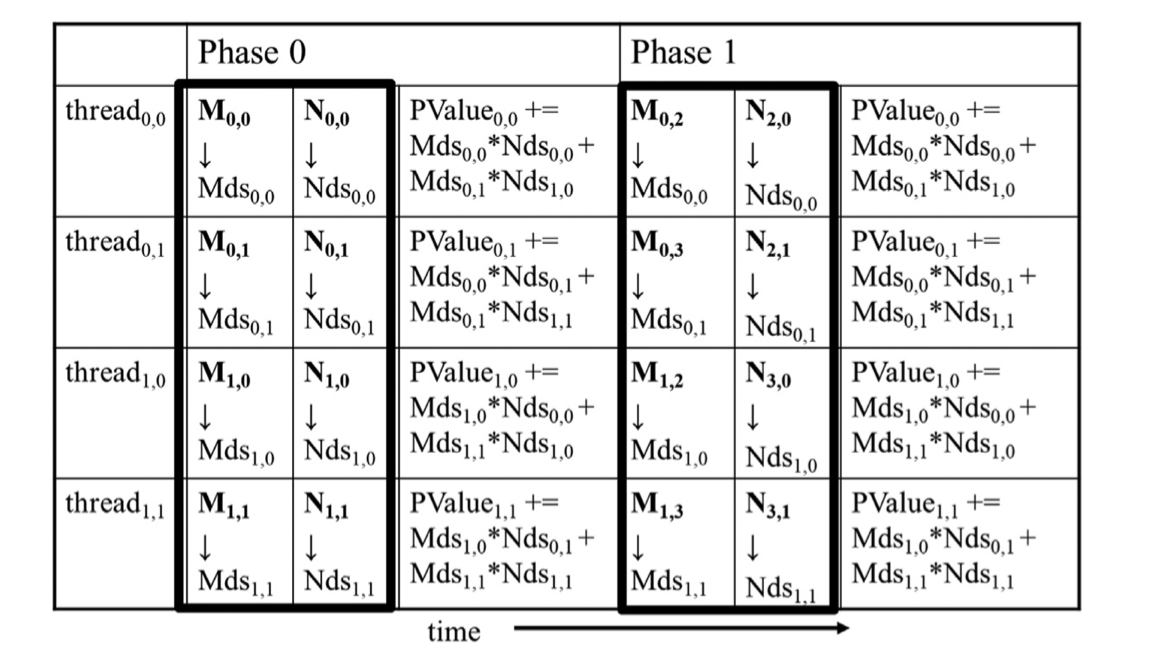
\includegraphics[width=0.9\textwidth]{figs/F5.8.png}
	\caption{\textit{定义为 lambda 的异步处理程序实现示例}}
\end{figure}

异步处理程序作为 std::function 传递到上下文或队列构造函数,
并且可以根据我们的偏好以常规函数、lambda 表达式或函数对象等方式进行定义。 
该处理程序必须接受 sycl::exception\_list 参数,如图 5-8 所示的示例处理程序所示。

在图 5-8 中,std::rethrow\_exception 后跟特定异常类型的 catch 提供了异常类型的过滤,
在本例中仅过滤 sycl::exception。 我们还可以使用 C++ 中的替代过滤方法,或者只选择处理所有异常,无论其类型如何。

处理程序在构造时与队列或上下文相关联(第 6 章中详细介绍了低级细节)。 
例如,要将图 5-8 中定义的处理程序注册到我们正在创建的队列中,我们可以编写

queue my\_queue\{ gpu\_selector\_v, handle\_async\_error \};

同样,要将图 5-8 中定义的处理程序注册到我们正在创建的上下文中,我们可以编写

context my\_context\{handle\_async\_error \};

大多数应用程序不需要显式创建或管理上下文(它们是在后台自动为我们创建的),
因此如果要使用异步处理程序,大多数开发人员应该将此类处理程序与为特定设备构建的队列相关联 (而不是明确的上下文)。

\begin{remark}
	在定义异步处理程序时,大多数开发人员应该在队列上定义它们,除非出于其他原因已经显式管理上下文。
\end{remark}

\begin{figure}[H]
	\centering
	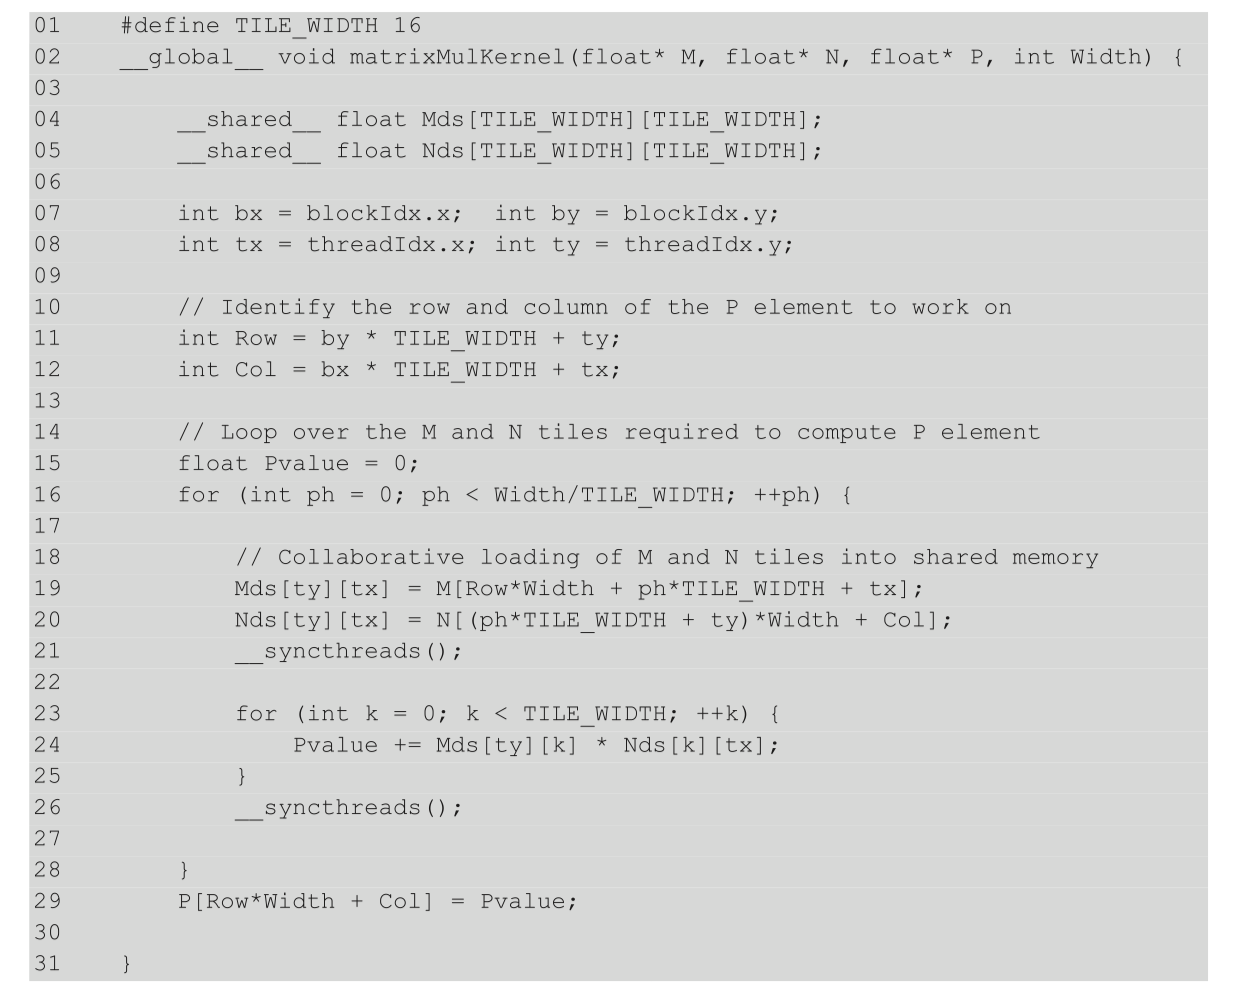
\includegraphics[width=0.9\textwidth]{figs/F5.9.png}
	\caption{\textit{默认异步处理程序的行为示例}}
\end{figure}

如果没有为队列或队列的父上下文定义异步处理程序,并且该队列(或上下文)发生必须处理的异步错误,则调用默认异步处理程序。 
默认处理程序的运行方式就好像它的编码如图 5-9 所示。

默认处理程序应向用户显示有关异常列表中任何错误的一些信息,
然后通过 std::terminate 结束应用程序,这应导致操作系统报告终止异常。

我们在异步处理程序中放置的内容取决于我们。 
它的范围可以从记录错误到应用程序终止,再到恢复错误条件以便应用程序可以继续正常执行。 
常见情况是通过调用 sycl::exception::what() 报告可用错误的任何详细信息,然后终止应用程序。

虽然异步处理程序在内部做什么由我们决定,但一个常见的错误是打印一条错误消息(可能会在程序中的其他消息的噪音中错过),
然后完成处理程序函数。 除非我们制定了错误管理原则,允许我们恢复已知的程序状态并确信继续执行是安全的,
否则我们应该考虑在异步处理程序函数中终止应用程序。 
这减少了检测到错误但无意中允许应用程序继续执行的程序出现错误结果的机会。 
在许多程序中,一旦我们检测到异步异常,异常终止是首选结果。

\begin{remark}
	如果未建立全面的错误恢复和管理机制,请考虑在输出有关错误的信息后终止异步处理程序中的应用程序。
\end{remark}

\subsubsection{处理程序的调用}
异步处理程序由运行时在特定时间调用。 
错误发生时不会立即报告,因为如果是这种情况,错误管理和安全应用程序编程(特别是多线程)
将变得更加困难和昂贵(例如,主机和设备之间的额外同步)。 相反,异步处理程序会在以下特定时间被调用:

\begin{enumerate}
	\item 当主机程序对特定队列调用queue::throw\_asynchronous()时

	\item 当主机程序对特定队列调用queue::wait\_and\_throw()时

	\item 当主机程序对特定事件调用 event::wait\_and\_throw() 时

	\item 当队列被销毁时

	\item 当上下文被破坏时
\end{enumerate}

方法 1-3 为主机程序提供了一种控制何时处理异步异常的机制,以便可以管理线程安全和特定于应用程序的其他细节。 
它们有效地提供了异步异常进入主机程序控制流的控制点,并且几乎可以像处理同步错误一样进行处理。

如果用户没有显式调用方法 1-3 之一,则在程序拆卸过程中,当队列和上下文被销毁时,通常会报告异步错误。 
这通常足以向用户发出信号,表明出现了问题并且程序结果不值得信任。

然而,依靠程序拆卸期间的错误检测并不适用于所有情况。 
例如,如果程序仅在达到某些算法收敛标准时才会终止,并且这些标准只能通过成功执行设备Kernel才能实现,
则异步异常可能表明该算法永远不会收敛并开始拆卸(其中错误 会被注意到)。 
在这些情况下,以及在制定了更完整的错误处理策略的生产应用程序中,
在程序中的常规和受控点调用 throw\_asynchronous() 
或 wait\_and\_throw() 是有意义的(例如,在检查算法是否收敛之前) 。

\subsection{设备上的错误}
本章讨论的错误检测和处理机制是基于主机的。 
它们是主机程序可以检测和处理主机程序中或在设备上执行Kernel期间可能出现问题的机制。 
我们没有讨论的是如何从我们编写的设备代码中发出信号,表明出现了问题。 这种遗漏并不是错误,而是故意的。

SYCL 明确不允许在设备代码中使用 C++ 异常处理机制(例如 throw),因为某些类型的设备会产生我们通常不想支付的性能成本。 
如果我们检测到设备代码中出现问题,我们应该使用现有的非基于异常的技术来发出错误信号。 
例如,我们可以写入一个缓冲区来记录错误或从我们定义的数值计算中返回一些无效结果,这些结果意味着发生了错误。 
在这些情况下,正确的策略是非常具体的应用程序。

\subsection{总结}
在本章中,我们介绍了同步和异步错误,介绍了如果我们不采取任何措施来管理可能发生的错误时预期的默认行为,
并介绍了用于在应用程序中的受控点处理异步错误的机制。 
错误管理策略是软件工程中的一个主要主题,并且在许多应用程序中编写的代码中占很大比例。 
SYCL 集成了我们在错误处理方面已有的 C++ 知识,并提供了灵活的机制来与我们首选的错误管理策略集成。